\documentclass{article}
\usepackage[paper=letterpaper,margin=2cm]{geometry}
\usepackage[russian]{babel}
\usepackage[utf8]{inputenc}
\usepackage[]{graphicx}
\usepackage[usenames]{color}
\usepackage{colortbl}
\usepackage{geometry}
\usepackage{xcolor}
\usepackage{listings}

\geometry{
  a4paper,
  top=25mm, 
  right=30mm, 
  bottom=25mm, 
  left=30mm
}

\begin{document}

\begin{center}
  \section*{
    Федеральное государственное автономное образовательное учреждение\\ высшего образования\\
    «Национальный исследовательский университет ИТМО»\\
    Факультет Программной Инженерии и Компьютерной Техники \\
   }
  
\includegraphics[scale=0.2]{../../img/itmo.png}
\end{center}
\vspace{4cm}


\begin{center}
  \large \textbf{Вариант \textnumero 311517}\\
  \textbf{Лабораторная работа \textnumero 1}\\
  по дисциплине\\
  \textbf{Основы профессиональной деятельности}
\end{center}

\vspace*{\fill}

\begin{flushright}
  Выполнил Студент группы P3115\\
  \textbf{Владимир Мацюк}\\
  Преподаватель: \\
  \textbf{ФИО препода}\\
\end{flushright}

\vspace{1cm}

\begin{center}
  г. Санкт-Петербург\\
  2022г.
\end{center}

\newpage

\lstset{
  inputencoding=utf8,
  frame=single,
  language=bash,
  breaklines=true,
  extendedchars=false,
  showspaces=false,
  showstringspaces=false,
  basicstyle=\footnotesize\ttfamily,
  keywordstyle=\bfseries\color{green!40!black},
  commentstyle=\itshape\color{purple!40!black},
  identifierstyle=\color{blue},
  stringstyle=\color{orange},
}

\section*{Цель работы}
Знакомство с основным способом взаимодействия с ОС UNIX,
командным интерфейсом, а также базовой функциональностью
интерпретатора shell. Получение основных сведений о файловой
системе и правах доступа к файлам.

\section*{Ход работы}

% Part 1

1. Создать приведенное в варианте дерево каталогов и файлов с содержимым. В качестве корня дерева использовать каталог lab0 своего домашнего каталога. Для создания и навигации по дереву использовать команды: mkdir, echo, cat, touch, ls, pwd, cd, more, cp, rm, rmdir, mv.

\vspace*{\fill}
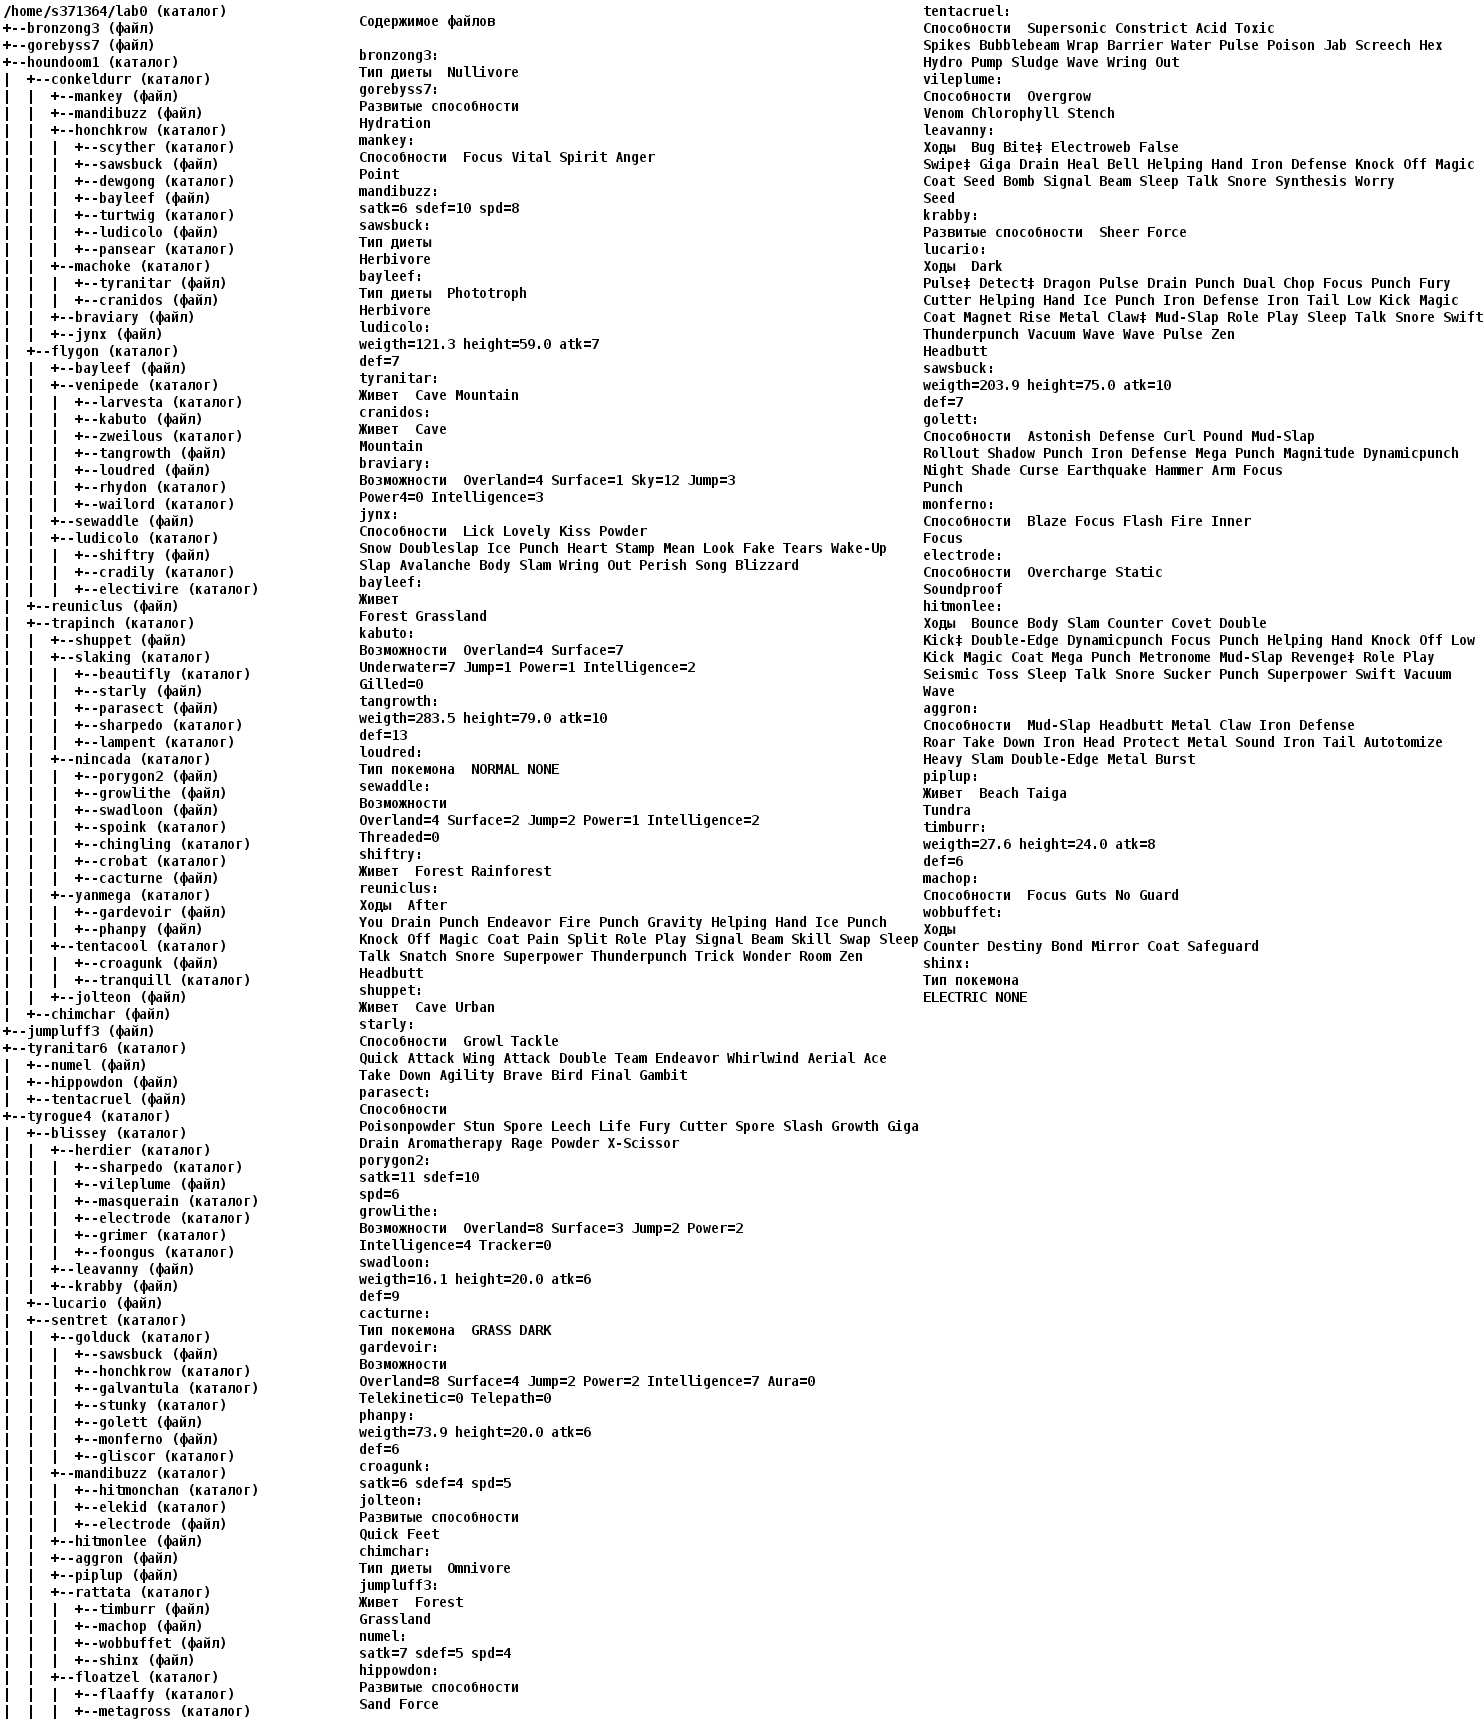
\includegraphics[width=\textwidth]{files.png}

\begin{lstlisting}
echo $'Тип диеты Nullivore' > bronzong3
echo $'Развитые способности\nHydration' > gorebyss7
mkdir houndoom1 && cd $_
  mkdir conkeldurr && cd $_
    echo $'Способности Focus Vital Spirit Anger\nPoint' > mankey
    echo $'satk=6 sdef=10 spd=8' > mandibuzz
    mkdir honchkrow && cd $_
      mkdir scyther
      echo $'Тип диеты\nHerbivore' > sawsbuck
      mkdir dewgong
      echo $'Тип диеты Phototroph\nHerbivore' > bayleef
      mkdir turtwig
      echo $'weigth=121.3 height=59.0 atk=7\ndef=7' > ludicolo
      mkdir pansear && cd ..
    mkdir machoke && cd $_
      echo $'Живет Cave Mountain' > tyranitar
      echo $'Живет Cave\nMountain' > cranidos && cd ..
    echo $'Возможности Overland=4 Surface=1 Sky=12 Jump=3\nPower4=0 Intelligence=3' > braviary
    echo $'Способности Lick lovely Kiss Powder\nSnow Doubleslap Ice Punch Heart Stamp Mean Look Fake Tears Wake-Up\nSlap Avalanche Body Slam Wring Out Perish Song Blizzard' > jynx && cd ..
  mkdir flygon && cd $_
    echo $'Живет\nForest Grassland' > bayleef
    mkdir venipede && cd $_
      mkdir larvesta
      echo $'Возможности Overland=4 Surface=7\nUnderwater=7 Jump=1 Power=1 Intelligence=2\nGilled=0' > kabuto
      mkdir zweilous
      echo $'weigth=283.5 height=79.0 atk=10\ndef=13' > tangrowth
      echo $'Тип покемона NORMAL NONE' > loudred
      mkdir rhydon
      mkdir wailord && cd ..
    echo $'Возможности\nOverland=4 Surface=2 Jump=2 Power=1 Intelligence=2\nThreaded=0' > sewaddle 
    mkdir ludicolo && cd $_
      echo $'Живет Forest Rainforest' > shiftry
      mkdir cradily
      mkdir electivire && cd ..
      cd ..
  echo $'Холы After\nYou Drain Punch Endeavor Fire Punch Gravity Helping Hand Ice Punch\nKnock Off Magic Coat Pain Split Role Play Signal Beam Skill Swap Sleep\nTalk Snatch Snore Superpower Thunderpunch Trick Wonder Room Zen\nHeadbutt' > reuniclus
  mkdir trapinch && cd $_
    echo $'Живет Cave Urban' > shuppet
    mkdir slaking && cd $_
      mkdir beautifly
      echo $'Способности Growl Tackle\nQuick Attack Wing Attack Double Team Endeavor whirlwind Aerial Ace\nTake Down Agility Brave Bird Final Gambit' > starly
      echo $'Способности\nPoisonpowder Stun Spore Leech Life Fury Cutter Spore Slash Growth Giga\nDrain Aromatherapy Rage Powder X-Scissor' > parasect
      mkdir sharpedo
      mkdir lampent && cd ..
    mkdir nincada && cd $_
      echo $'satk=11 sdef=10\nspd=6' > porygon2
      echo $'Возможности Overland=8 Surface=3 Jump=2 Power=2\nIntelligence=4 Tracker=0' > growlithe
      echo $'weigth=16.1 height=20.0 atk=6\ndef=9' > swadloon
      mkdir spoink
      mkdir chingling
      mkdir crobat
      echo $'Тип покемона GRASS DARK' > cacturne && cd ..
    mkdir yanmega && cd $_
      echo $'Возможности\nOverland=8 Surface=4 Jump=2 Power=2 Intelligence=7 Aura=0\nTelekinetic=0 Telepath=0' > gardevoir
      echo $'weigth=73.9 height=20.0 atk=6\ndef=6' > phanpy && cd ..
    mkdir tentacool && cd $_
      echo $'satk=6 sdef=4 spd=5' > croagunk
      mkdir tranquill && cd ..
    echo $'Развитые способности\nQuick Feet' > jolteon && cd ..
  echo $'Тип диеты Omnivore' > chimchar && cd ..
echo $'Живет Forest\nGrassland' > jumpluff3
mkdir tyranitar6 && cd $_
  echo $'satk=7 sdef=5 spd=4' > numel
  echo $'Развитые способности\nSand Force' > hippowdon
  echo $'Способности Supersonic Constrict Acid Toxic\nSpikes Bubblebean Wrap Barrier Water Pulse Poison Jab Screech Hex\nHydro Pump Sludge Wave Wring Out' > tentacruel && cd ..
mkdir tyrogue4 && cd $_
  mkdir blissey && cd $_
    mkdir herdier && cd $_
      mkdir sharpedo
      echo $'Способности Overgrow\nVenom Chlorophyll Stench' > vileplume
      mkdir masquerain
      mkdir electrode
      mkdir grimer
      mkdir foongus && cd ..
    echo $'Ходы Bug Bitet Electroweb False\nSwipet Giga Drain Heal Bell Helping Hand Iron Defense Knock Off Magic Coat Seed Bomb Signal Beam Sleep Talk Snore Synthesis\nWorry\nSeed' > leavanny
    echo $'Развитые способности Sheer Force' > krabby && cd ..
  echo $'Ходы Dark\nPulset‡ Detect!‡Dragon Pulse Drain Punch Dual Chop Focus Punch Fury\nCutter Helping Hand Ice Punch Iron Defense Iron Tail Low Kick Magic\nCoat Magnet Rise Metal Claw‡ Mud-Slap Role Play Sleep Talk Snore Swift\nThunderpunch Vacuum Wave Wave Pulse Zen\nHeadbutt' > lucario
  mkdir sentret && cd $_
    mkdir golduck && cd $_
      echo $'weigth=203.9 height=75.0 atk=10\ndef=7' > sawsbuck
      mkdir honchkrow
      mkdir galvantula
      mkdir stunky
      echo $'Способности Astonish Defense Curl Pound Mud-Slap\nRollout Shadow Punch Iron Defense Mega Punch Magnitude Dynamicpunch\nNight Shade Curse Earthquake Hammer Arm Focus\nPunch' > golett
      echo $'Способности Blaze Focus Flash Fire Inner\nFocus' > monferno
      mkdir gliscor && cd ..
    mkdir mandibuzz && cd $_
      mkdir hitmonchan
      mkdir elekid
      echo $'Способности Overcharge Static\nSoundproof' > electrode && cd ..
    echo $'Ходы Bounce Body Slam Counter Covet Double\nKick‡ Double-Edge Dynamicpunch Focus Punch Helping Hand Knock Off Low\nKick Magic Coat Mega Punch Metronome Hud-Slap Revenge Role Play\nSeismic Toss Sleep Talk Snore Sucker Punch Superpower Swift Vacuum\nWave' > hitmonlee
    echo $'Способности Mud-Slap Headbutt Metal Claw Iron Defense\nRoar Take Down Iron Head Protect Metal Sound Iron Tail Autotomize\nHeavy Slam Double-Edge Metal Burst' > aggron
    echo $'Живет Beach Taiga\nTundra' > piplup
    mkdir rattata && cd $_
      echo $'weigth=27.6 height=24.0 atk=8\ndef=6' > timburr
      echo $'Способности Focus Guts No Guard' > machop
      echo $'Ходы\nCounter Destiny Bond Mirror Coat Safeguard' > wobbuffet
      echo $'Тип покемона\nELECTRIC NONE' > shinx && cd ..
    mkdir floatzel && cd $_
      mkdir flaaffy
      mkdir metagross && cd ..
    cd ..
  cd ..
\end{lstlisting}
\newpage

% Part 2
2. Установить согласно заданию права на файлы и каталоги при помощи команды chmod, используя различные способы указания прав.

\begin{itemize}
  \item bronzong3: владелец должен читать и записывать файл; группа-владелец должна не иметь никаких прав; остальные пользователи должны читать файл
  \item gorebyss7: владелец должен читать файл; группа-владелец должна не иметь никаких прав; остальные пользователи должны не иметь никаких прав
  \item houndoom1: -wxrw--wx
  \item conkeldurr: владелец должен читать, записывать директорию и переходить в нее; группа-владелец должна читать, записывать директорию и переходить в нее; остальные пользователи должны читать, записывать директорию и переходить в нее
  \item mankey: права 064
  \item mandibuzz: права 600
  \item honchkrow: права 571
  \item scyther: права 317
  \item sawsbuck: владелец должен не иметь никаких прав; группа-владелец должна читать файл; остальные пользователи должны читать и записывать файл
  \item dewgong: r-x--x-w-
  \item bayleef: права 444
  \item turtwig: владелец должен читать, записывать директорию и переходить в нее; группа-владелец должна читать директорию и переходить в нее; остальные пользователи должны записывать директорию и переходить в нее
  \item ludicolo: владелец должен не иметь никаких прав; группа-владелец должна не иметь никаких прав; остальные пользователи должны читать и записывать файл
  \item pansear: -wxrwxr-x
  \item machoke: r-x-w-r--
  \item tyranitar: права 440
  \item cranidos: владелец должен не иметь никаких прав; группа-владелец должна читать файл; остальные пользователи должны читать файл
  \item braviary: владелец должен читать и записывать файл; группа-владелец должна записывать файл; остальные пользователи должны записывать файл
  \item jynx: rw--w-r--
  \item flygon: -wx-wxr-x
  \item bayleef: владелец должен читать файл; группа-владелец должна не иметь никаких прав; остальные пользователи должны не иметь никаких прав
  \item venipede: владелец должен читать директорию и переходить в нее; группа-владелец должна только переходить в директорию; остальные пользователи должны записывать директорию
  \item larvesta: rwxr-x-w-
  \item kabuto: права 404
  \item zweilous: права 770
  \item tangrowth: r--------
  \item loudred: владелец должен не иметь никаких прав; группа-владелец должна читать файл; остальные пользователи должны читать файл
  \item rhydon: r-xrwx-wx
  \item wailord: владелец должен читать, записывать директорию и переходить в нее; группа-владелец должна записывать директорию и переходить в нее; остальные пользователи должны читать и записывать директорию
  \item sewaddle: ---r--rw-
  \item ludicolo: владелец должен читать директорию и переходить в нее; группа-владелец должна записывать директорию и переходить в нее; остальные пользователи должны читать, записывать директорию и переходить в нее
  \item shiftry: права 404
  \item cradily: rwxr-x-wx
  \item electivire: rwx-wx-wx
  \item reuniclus: права 600
  \item trapinch: права 357
  \item shuppet: r--r--r--
  \item slaking: права 330
  \item beautifly: права 500
  \item starly: rw--w----
  \item parasect: ---rw----
  \item sharpedo: -wxrw---x
  \item lampent: r-x-wxrwx
  \item nincada: права 305
  \item porygon2: ---rw----
  \item growlithe: r--r--r--
  \item swadloon: rw--w-r--
  \item spoink: -wxrwx-wx
  \item chingling: владелец должен читать директорию и переходить в нее; группа-владелец должна только переходить в директорию; остальные пользователи должны записывать директорию и переходить в нее
  \item crobat: владелец должен записывать директорию и переходить в нее; группа-владелец должна читать, записывать директорию и переходить в нее; остальные пользователи должны читать директорию и переходить в нее
  \item cacturne: права 664
  \item yanmega: r-x--x-wx
  \item gardevoir: ---r--r--
  \item phanpy: владелец должен читать и записывать файл; группа-владелец должна записывать файл; остальные пользователи должны читать файл
  \item tentacool: права 337
  \item croagunk: rw-------
  \item tranquill: права 771
  \item jolteon: владелец должен не иметь никаких прав; группа-владелец должна читать файл; остальные пользователи должны читать файл
  \item chimchar: владелец должен читать файл; группа-владелец должна читать файл; остальные пользователи должны читать файл
  \item jumpluff3: права 004
  \item tyranitar6: права 305
  \item numel: владелец должен читать файл; группа-владелец должна не иметь никаких прав; остальные пользователи должны читать файл
  \item hippowdon: владелец должен не иметь никаких прав; группа-владелец должна не иметь никаких прав; остальные пользователи должны читать файл
  \item tentacruel: r--------
  \item tyrogue4: владелец должен читать директорию и переходить в нее; группа-владелец должна записывать директорию и переходить в нее; остальные пользователи должны читать, записывать директорию и переходить в нее
  \item blissey: владелец должен читать директорию и переходить в нее; группа-владелец должна только переходить в директорию; остальные пользователи должны записывать директорию
  \item herdier: владелец должен читать директорию и переходить в нее; группа-владелец должна читать, записывать директорию и переходить в нее; остальные пользователи должны читать, записывать директорию и переходить в нее
  \item sharpedo: rwxrwxrwx
  \item vileplume: ---r--rw-
  \item masquerain: права 755
  \item electrode: rwx-wx-wx
  \item grimer: владелец должен читать директорию и переходить в нее; группа-владелец должна читать, записывать директорию и переходить в нее; остальные пользователи должны записывать директорию и переходить в нее
  \item foongus: владелец должен читать директорию и переходить в нее; группа-владелец должна читать, записывать директорию и переходить в нее; остальные пользователи должны записывать директорию и переходить в нее
  \item leavanny: владелец должен читать файл; группа-владелец должна не иметь никаких прав; остальные пользователи должны не иметь никаких прав
  \item krabby: права 600
  \item lucario: rw-r-----
  \item sentret: права 355
  \item golduck: владелец должен читать директорию и переходить в нее; группа-владелец должна читать, записывать директорию и переходить в нее; остальные пользователи должны записывать директорию и переходить в нее
  \item sawsbuck: ---r--rw-
  \item honchkrow: права 500
  \item galvantula: права 771
  \item stunky: права 555
  \item golett: rw----r--
  \item monferno: владелец должен не иметь никаких прав; группа-владелец должна не иметь никаких прав; остальные пользователи должны читать файл
  \item gliscor: владелец должен читать, записывать директорию и переходить в нее; группа-владелец должна записывать директорию и переходить в нее; остальные пользователи должны читать и записывать директорию
  \item mandibuzz: r-xrwxrwx
  \item hitmonchan: владелец должен читать, записывать директорию и переходить в нее; группа-владелец должна записывать директорию и переходить в нее; остальные пользователи должны читать и записывать директорию
  \item elekid: владелец должен читать, записывать директорию и переходить в нее; группа-владелец должна записывать директорию и переходить в нее; остальные пользователи должны записывать директорию и переходить в нее
  \item electrode: владелец должен читать и записывать файл; группа-владелец должна читать файл; остальные пользователи должны не иметь никаких прав
  \item hitmonlee: права 640
  \item aggron: права 404
  \item piplup: права 600
  \item rattata: права 555
  \item timburr: права 664
  \item machop: r-----r--
  \item wobbuffet: r--r--r--
  \item shinx: владелец должен читать файл; группа-владелец должна не иметь никаких прав; остальные пользователи должны не иметь никаких прав
  \item floatzel: владелец должен читать, записывать директорию и переходить в нее; группа-владелец должна читать директорию и переходить в нее; остальные пользователи должны записывать директорию
  \item flaaffy: права 711
  \item metagross: права 570
\end{itemize}


\begin{lstlisting}
chmod u=rw,g=,o=r        bronzong3
chmod u=r,g=,o=          gorebyss7
chmod u=wx,g=rw,o=wx     houndoom1
chmod u=rwx,g=rwx,o=rwx  houndoom1/conkeldurr
chmod 064                houndoom1/conkeldurr/mankey
chmod 600                houndoom1/conkeldurr/mandibuzz
chmod 571                houndoom1/conkeldurr/honchkrow
chmod 317                houndoom1/conkeldurr/honchkrow/scyther
chmod u=,g=r,o=rw        houndoom1/conkeldurr/honchkrow/sawsbuck
chmod u=rx,g=x,o=w       houndoom1/conkeldurr/honchkrow/dewgong
chmod 444                houndoom1/conkeldurr/honchkrow/bayleef
chmod u=rwx,g=rx,o=wx    houndoom1/conkeldurr/honchkrow/turtwig
chmod u=,g=,o=rw         houndoom1/conkeldurr/honchkrow/ludicolo
chmod u=wx,g=rwx,o=rx    houndoom1/conkeldurr/honchkrow/pansear
chmod u=rx,g=w,o=r       houndoom1/conkeldurr/machoke
chmod 440                houndoom1/conkeldurr/machoke/tyranitar
chmod u=,g=r,o=r         houndoom1/conkeldurr/machoke/cranidos
chmod u=rw,g=w,o=w       houndoom1/conkeldurr/braviary
chmod u=rw,g=w,o=r       houndoom1/conkeldurr/jynx
chmod u=wx,g=wx,o=rx     houndoom1/flygon
chmod u=r,g=,o=          houndoom1/flygon/bayleef
chmod u=rx,g=x,o=w       houndoom1/flygon/venipede
chmod u=rwx,g=rx,o=w     houndoom1/flygon/venipede/larvesta
chmod 404                houndoom1/flygon/venipede/kabuto
chmod 770                houndoom1/flygon/venipede/zweilous
chmod u=r,g=,o=          houndoom1/flygon/venipede/tangrowth
chmod u=,g=r,o=r         houndoom1/flygon/venipede/loudred
chmod u=rx,g=rwx,o=wx    houndoom1/flygon/venipede/rhydon
chmod u=rwx,g=wx,o=rw    houndoom1/flygon/venipede/wailord
chmod u=,g=r,o=rw        houndoom1/flygon/sewaddle
chmod u=rx,g=wx,o=rwx    houndoom1/flygon/ludicolo
chmod 404                houndoom1/flygon/ludicolo/shiftry
chmod u=rwx,g=rx,o=wx    houndoom1/flygon/ludicolo/cradily
chmod u=rwx,g=wx,o=wx    houndoom1/flygon/ludicolo/electivire
chmod 600                houndoom1/reuniclus
chmod 357                houndoom1/trapinch
chmod u=r,g=r,o=r        houndoom1/trapinch/shuppet
chmod 330                houndoom1/trapinch/slaking
chmod 500                houndoom1/trapinch/slaking/beautifly
chmod u=rw,g=w,o=        houndoom1/trapinch/slaking/starly
chmod u=,g=rw,o=         houndoom1/trapinch/slaking/parasect
chmod u=wx,g=rw,o=x      houndoom1/trapinch/slaking/sharpedo
chmod u=rx,g=wx,o=rwx    houndoom1/trapinch/slaking/lampent
chmod 305                houndoom1/trapinch/nincada
chmod u=,g=rw,o=         houndoom1/trapinch/nincada/porygon2
chmod u=r,g=r,o=r        houndoom1/trapinch/nincada/growlithe
chmod u=rw,g=w,o=r       houndoom1/trapinch/nincada/swadloon
chmod u=wx,g=rwx,o=wx    houndoom1/trapinch/nincada/spoink
chmod u=rx,g=x,o=wx      houndoom1/trapinch/nincada/chingling
chmod u=wx,g=rwx,o=rx    houndoom1/trapinch/nincada/crobat
chmod 664                houndoom1/trapinch/nincada/cacturne
chmod u=rx,g=x,o=wx      houndoom1/trapinch/yanmega
chmod u=,g=r,o=r         houndoom1/trapinch/yanmega/gardevoir
chmod u=rw,g=w,o=r       houndoom1/trapinch/yanmega/phanpy
chmod 337                houndoom1/trapinch/tentacool
chmod u=rw,g=,o=         houndoom1/trapinch/tentacool/croagunk
chmod 771                houndoom1/trapinch/tentacool/tranquill
chmod u=,g=r,o=r         houndoom1/trapinch/jolteon
chmod u=r,g=r,o=r        houndoom1/chimchar
chmod 004                jumpluff3
chmod 305                tyranitar6
chmod u=r,g=,o=r         tyranitar6/numel
chmod u=,g=,o=r          tyranitar6/hippowdon
chmod u=r,g=,o=          tyranitar6/tentacruel
chmod u=rx,g=wx,o=rwx    tyrogue4
chmod u=rx,g=x,o=w       tyrogue4/blissey
chmod u=rx,g=rwx,o=rwx   tyrogue4/blissey/herdier
chmod u=rwx,g=rwx,o=rwx  tyrogue4/blissey/herdier/sharpedo
chmod u=,g=r,o=rw        tyrogue4/blissey/herdier/vileplume
chmod 755                tyrogue4/blissey/herdier/masquerain
chmod u=rwx,g=wx,o=wx    tyrogue4/blissey/herdier/electrode
chmod u=rx,g=rwx,o=wx    tyrogue4/blissey/herdier/grimer
chmod u=rx,g=rwx,o=wx    tyrogue4/blissey/herdier/foongus
chmod u=r,g=,o=          tyrogue4/blissey/leavanny
chmod 600                tyrogue4/blissey/krabby
chmod u=rw,g=r,o=        tyrogue4/lucario
chmod 355                tyrogue4/sentret
chmod u=rx,g=rwx,o=wx    tyrogue4/sentret/golduck
chmod u=,g=r,o=rw        tyrogue4/sentret/golduck/sawsbuck
chmod 500                tyrogue4/sentret/golduck/honchkrow
chmod 771                tyrogue4/sentret/golduck/galvantula
chmod 555                tyrogue4/sentret/golduck/stunky
chmod u=rw,g=,o=r        tyrogue4/sentret/golduck/golett
chmod u=,g=,o=r          tyrogue4/sentret/golduck/monferno
chmod u=rwx,g=wx,o=rw    tyrogue4/sentret/golduck/gliscor
chmod u=rx,g=rwx,o=rwx   tyrogue4/sentret/mandibuzz
chmod u=rwx,g=wx,o=rw    tyrogue4/sentret/mandibuzz/hitmonchan
chmod u=rwx,g=wx,o=wx    tyrogue4/sentret/mandibuzz/elekid
chmod u=rw,g=r,o=        tyrogue4/sentret/mandibuzz/electrode
chmod 640                tyrogue4/sentret/hitmonlee
chmod 404                tyrogue4/sentret/aggron
chmod 600                tyrogue4/sentret/piplup
chmod 555                tyrogue4/sentret/rattata
chmod 664                tyrogue4/sentret/rattata/timburr
chmod u=r,g=,o=r         tyrogue4/sentret/rattata/machop
chmod u=r,g=r,o=r        tyrogue4/sentret/rattata/wobbuffet
chmod u=r,g=,o=          tyrogue4/sentret/rattata/shinx
chmod u=rwx,g=rx,o=w     tyrogue4/sentret/floatzel
chmod 711                tyrogue4/sentret/floatzel/flaaffy
chmod 570                tyrogue4/sentret/floatzel/metagross
\end{lstlisting}
\newpage

% Part 3

3. Скопировать часть дерева и создать ссылки внутри дерева согласно заданию при помощи команд cp и ln, а также комманды cat и перенаправления ввода-вывода.

\begin{itemize}
  \item cоздать жесткую ссылку для файла jumpluff3 с именем lab0/tyrogue4/blissey/krabbyjumpluff
  \item cоздать символическую ссылку для файла bronzong3 с именем lab0/tyranitar6/numelbronzong
  \item создать символическую ссылку c именем Copy\_56 на директорию tyrogue4 в каталоге lab0
  \item скопировать файл jumpluff3 в директорию lab0/houndoom1/trapinch/tentacool
  \item скопировать файл jumpluff3 в директорию lab0/houndoom1/trapinch/nincada/chingling
  \item объеденить содержимое файлов lab0/houndoom1/reuniclus, lab0/tyrogue4/blissey/leavanny, lab0/tyrogue4/sentret/rattata/timburr, lab0/houndoom1/trapinch/nincada/porygon2, в новый файл lab0/bronzong3\_30
  \item cоздать жесткую ссылку для файла bronzong3 с именем lab0/houndoom1/flygon/venipede/loudredbronzong
  \item скопировать рекурсивно директорию houndoom1 в директорию lab0/houndoom1/trapinch/nincada
  \item скопировать содержимое файла gorebyss7 в новый файл lab0/houndoom1/trapinch/yanmega/phanpygorebyss
  \item объеденить содержимое файлов lab0/houndoom1/trapinch/nincada/growlithe, lab0/tyranitar6/tentacruel, lab0/houndoom1/trapinch/nincada/swadloon, lab0/houndoom1/flygon/ludicolo/shiftry, в новый файл lab0/gorebyss7\_25
  \item cоздать символическую ссылку для файла gorebyss7 с именем lab0/houndoom1/trapinch/jolteongorebyss
  \item скопировать содержимое файла jumpluff3 в новый файл lab0/houndoom1/trapinch/yanmega/gardevoirjumpluff
  \item cоздать жесткую ссылку для файла bronzong3 с именем lab0/tyranitar6/numelbronzong
  \item скопировать файл gorebyss7 в директорию lab0/houndoom1/flygon/venipede/rhydon
  \item объеденить содержимое файлов lab0/houndoom1/conkeldurr/honchkrow/bayleef, lab0/houndoom1/trapinch/slaking/starly, lab0/houndoom1/trapinch/yanmega/gardevoir, lab0/houndoom1/trapinch/nincada/porygon2, в новый файл lab0/bronzong3\_60
  \item скопировать рекурсивно директорию tyranitar6 в директорию lab0/tyrogue4/sentret/floatzel/flaaffy
  \item cоздать символическую ссылку для файла bronzong3 с именем lab0/houndoom1/conkeldurr/machoke/tyranitarbronzong
  \item скопировать рекурсивно директорию tyranitar6 в директорию lab0/houndoom1/flygon/venipede
  \item скопировать содержимое файла gorebyss7 в новый файл lab0/houndoom1/trapinch/yanmega/phanpygorebyss
  \item создать символическую ссылку c именем Copy\_56 на директорию tyranitar6 в каталоге lab0
  \item создать символическую ссылку c именем Copy\_22 на директорию tyranitar6 в каталоге lab0
\end{itemize}

\begin{lstlisting}
ln jumpluff3 tyrogue4/blissey/krabbyjumpluff
ln -s bronzong3 tyranitar6/numelbronzong
ln -s Copy_56 tyrogue4
cp jumpluff3 houndoom1/trapinch/tentacool
cp jumpluff3 houndoom1/trapinch/nincada/chingling
cat houndoom1/reuniclus tyrogue4/blissey/leavanny tyrogue4/sentret/rattata/timburr houndoom1/trapinch/nincada/porygon2 >> bronzong3_30
ln bronzong3 houndoom1/flygon/venipede/loudredbronzong
rsync -Rr houndoom1 houndoom1/trapinch/nincada  # use rsync because cp can't copy directory into itself
cp gorebyss7 houndoom1/trapinch/yanmega/phanpygorebyss
cat houndoom1/trapinch/nincada/growlithe tyranitar6/tentacruel houndoom1/trapinch/nincada/swadloon houndoom1/flygon/ludicolo/shiftry >> gorebyss7_25
ln -s gorebyss7 houndoom1/trapinch/jolteongorebyss
cp jumpluff3 houndoom1/trapinch/yanmega/gardevoirjumpluff
# ln bronzong3 tyranitar6/numelbronzong # symlink already exists (Part 3 second line)
cp gorebyss7 houndoom1/flygon/venipede/rhydon
cat houndoom1/conkeldurr/honchkrow/bayleef houndoom1/trapinch/slaking/starly houndoom1/trapinch/yanmega/gardevoir houndoom1/trapinch/nincada/porygon2 >> bronzong3_60
cp -r tyranitar6 tyrogue4/sentret/floatzel/flaaffy
ln -s bronzong3 houndoom1/conkeldurr/machoke/tyranitarbronzong
cp -r tyranitar6 houndoom1/flygon/venipede
cp gorebyss7 houndoom1/trapinch/yanmega/phanpygorebyss
ln -s Copy_56 tyranitar6
ln -s Copy_22 tyranitar6
\end{lstlisting}
\newpage

% Part 4
4. Используя команды cat, wc, ls, head, tail, echo, sort, grep выполнить в соответствии с вариантом задания поиск и фильтрацию файлов, каталогов и содержащихся в них данных.

\begin{itemize}
  \item Подсчитать количество символов содержимого файлов: numel, hippowdon, tentacruel, vileplume, leavanny, krabby, lucario, sawsbuck, golett, monferno, результат записать в файл в директории /tmp, подавить вывод ошибок доступа
  \item Вывести рекурсивно список имен и атрибутов файлов в директории lab0, содержащих строку "ke", список отсортировать по убыванию количества жестких ссылок, добавить вывод ошибок доступа в стандартный поток вывода
  \item Рекурсивно вывести содержимое файлов с номерами строк из директории lab0, имя которых начинается на 'l', строки отсортировать по имени a->z, подавить вывод ошибок доступа
  \item Вывести четыре первых элемента рекурсивного списка имен и атрибутов файлов в директории lab0, заканчивающихся на символ 'w', список отсортировать по возрастанию размера, ошибки доступа перенаправить в файл в директории /tmp
  \item Вывести три последних элемента рекурсивного списка имен и атрибутов файлов в директории lab0, содержащих строку "ke", список отсортировать по возрастанию даты доступа к файлу, подавить вывод ошибок доступа
  \item Вывести список имен и атрибутов файлов в директории houndoom1, список отсортировать по убыванию размера, ошибки доступа перенаправить в файл в директории /tmp
  \item Рекурсивно подсчитать количество строк содержимого файлов из директории lab0, имя которых заканчивается на 't', отсортировать вывод по уменьшению количества, подавить вывод ошибок доступа
  \item Подсчитать количество символов содержимого файла gorebyss7, результат записать в файл в директории /tmp, ошибки доступа перенаправить в файл в директории /tmp
  \item Вывести содержимое файла bronzong3 с номерами строк, оставить только строки, содержащие "rlan", регистр символов игнорировать, добавить вывод ошибок доступа в стандартный поток вывода
  \item Рекурсивно вывести содержимое файлов с номерами строк из директории lab0, имя которых заканчивается на 'k', строки отсортировать по имени a->z, добавить вывод ошибок доступа в стандартный поток вывода
  \item Вывести два последних элемента рекурсивного списка имен и атрибутов файлов в директории lab0, список отсортировать по возрастанию даты изменения записи о файле, добавить вывод ошибок доступа в стандартный поток вывода
  \item Вывести три последних элемента рекурсивного списка имен и атрибутов файлов в директории lab0, заканчивающихся на символ 'z', список отсортировать по имени z->a, ошибки доступа не подавлять и не перенаправлять
  \item Вывести рекурсивно список имен и атрибутов файлов в директории lab0, начинающихся на символ 'n', список отсортировать по возрастанию даты модификации файла, добавить вывод ошибок доступа в стандартный поток вывода
  \item Вывести два последних элемента рекурсивного списка имен и атрибутов файлов в директории lab0, содержащих строку "lo", список отсортировать по возрастанию размера, ошибки доступа не подавлять и не перенаправлять
  \item Рекурсивно вывести содержимое файлов из директории lab0, имя которых заканчивается на 'y', строки отсортировать по имени z->a, ошибки доступа не подавлять и не перенаправлять
  \item Вывести список имен файлов в директории tyranitar6, список отсортировать по имени z->a, ошибки доступа перенаправить в файл в директории /tmp
  \item Подсчитать количество строк содержимого файлов: jynx, bayleef, kabuto, tangrowth, loudred, sewaddle, shiftry, reuniclus, shuppet, starly, отсортировать вывод по увеличению количества, подавить вывод ошибок доступа
  \item Вывести список имен и атрибутов файлов в директории tyranitar6, список отсортировать по имени z->a, ошибки доступа перенаправить в файл в директории /tmp
\end{itemize}

\begin{lstlisting}
  wc -m ./{,*/,*/*/,*/*/*/,*/*/*/*/}{*numel,hippowdon,tentacruel,vileplume,leavanny,krabby,lucario,sawsbuck,golett,monferno} 2>/dev/null 1>/tmp/task1
  ls -ltuR 2>&1 | grep '\s[0-9a-zA-Z]*ke[0-9a-zA-Z]*$' | sort -k2 -r
cat -n ./{,*/,*/*/,*/*/*/,*/*/*/*/}l* 2>/dev/null | sort -k2
ls -ltuR 2>/tmp/task5_err | grep '\s[0-9a-zA-Z]*w$' | sort -k5 | head -n 4
ls -ltuR 2>/dev/null | grep '^\-.*\s[0-9a-zA-Z]*ke[0-9a-zA-Z]*$' | sort -k7 | tail -n 3
ls -lp houndoom1/ 2>/tmp/task6_err | grep -v / | sort -k5 -r
wc -l ./{,*/,*/*/,*/*/*/,*/*/*/*/}*t 2>/dev/null | sort  -r
wc -m gorebyss7 1>/tmp/task7 2>/tmp/task7_err
cat -n bronzong3 | grep -i rlan 2>&1
cat -n ./{,*/,*/*/,*/*/*/,*/*/*/*/}*k | sort -k2 2>&1
ls -ltuR 2>&1 | grep '\s[0-9a-zA-Z]*$' | sort -k8 | tail -n 2
ls -ltuR | grep '\s[0-9a-zA-Z]*z$' | sort -k9 -r | tail -n 3
ls -ltuR 2>&1 | grep '\sn[0-9a-zA-Z]*$' | sort -k8
ls -ltuR | grep '\s[0-9a-zA-Z]*lo[0-9a-zA-Z]*$' | sort -k5 | tail -n 2
cat ./{,*/,*/*/,*/*/*/,*/*/*/*/}*y | sort -r
ls tyranitar6/ 2>/tmp/task16_err | sort -r
wc -l ./{,*/,*/*/,*/*/*/,*/*/*/*/}{*jynx,bayleef,kabuto,tangrowth,loudred,sewaddle,shiftry,reuniclus,shuppet,starly} 2>/dev/null | sort
ls -l tyranitar6/ 2>/tmp/task18_err | sort -k9 -r
\end{lstlisting}

\newpage

% Part 5
5. Выполнить удаление файлов и каталогов при помощи команд rm и rmdir согласно варианту задания.

\begin{itemize}
  \item Удалить файл gorebyss7
  \item Удалить файл lab0/tyrogue4/sentret/rattata/wobbuffet
  \item удалить символические ссылки lab0/houndoom1/conkeldurr/machoke/tyranitarbronzo*
  \item удалить жесткие ссылки lab0/tyranitar6/numelbronzo*
  \item Удалить директорию tyranitar6
  \item Удалить директорию lab0/houndoom1/trapinch/nincada
\end{itemize}

\begin{lstlisting}
rm -f gorebyss7
rm -f tyrogue4/sentret/rattata/wobbuffet
rm houndoom1/conkeldurr/machoke/tyranitarbronzo*
rm tyranitar6/numelbronzo*
rm -Rf tyranitar6
rm -Rf houndoom1/trapinch/nincada
\end{lstlisting}

\vspace*{\fill}


\section*{Вывод}
Я познакомился с основным способом взаимодействия с ОС Linux,
командным интерфейсом, а также базовой функциональностью
интерпретатора shell и получил основные сведения о файловой
системе и правах доступа к файлам.
\end{document}
